\documentclass[12pt]{beamer}
\usepackage[T1]{fontenc}
\usepackage[utf8]{inputenc}
\usepackage[brazil]{babel}
\usepackage{graphicx}

\graphicspath{ {./../images/} }
\usetheme{Antibes}
\usecolortheme{default}

\usepackage{amssymb,amsmath}
\usepackage{textgreek}
\usepackage{tikz}
\usepackage{lipsum}

%\hypersetup {
%  pdftitle = {?},
%  pdfauthor = {?},
%  pdfsubject = {?},
%  pdfkeywords = {?}
%}

\setbeamertemplate{headline}{}
\setbeamertemplate{navigation symbols}{}

\title[Database]{Database}
\author{
  Mateus Siqueira Batista\and
  Nicolas Bissoli Nattis
}
\institute{
  MC536 - Instituto de Computação, UNICAMP
}
\date[2020]{2020}

\begin{document}

\frame{\titlepage}

\begin{frame}
  \frametitle{Proposta}
  Obter dados de interações entre genes e drogas, e entre genes e doenças.
  \pause

  Através disso, podemos relacionar a interação entre estas drogas e as doenças.
  \pause
  
  Por exemplo:
  \begin{itemize}
    \item Droga A ativa o gene X.
    \item Gene X codifica a proteína X.
    \item Proteína X tem relação de causa com as doenças \textalpha, \textgamma.
    \item Portanto, a droga A tem relação de causa com as doenças \textalpha, \textgamma.
  \end{itemize}
\end{frame}

\begin{frame}
  \frametitle{DGIdb}
  
\includegraphics[scale=0.8]{dgi.png}
  \begin{itemize}
    \item {Dados sobre interações droga-gene e o genoma drogável.}
    \item {Extraído de mais de trinta fontes confiáveis.}
  \end{itemize}
\end{frame} 

\begin{frame}
  \frametitle{DisGeNet}
  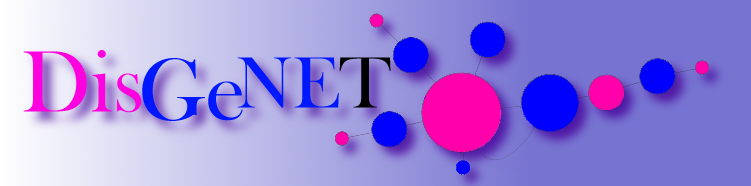
\includegraphics[scale=0.425]{disgenet.png}
  \begin{itemize}
    \item {Plataforma contendo uma das maiores coleções publicamente disponíveis de genes e variantes associados a doenças humanas.}
  \end{itemize}
\end{frame} 

\end{document}
